\documentclass{article}

\usepackage{color}
\usepackage{graphicx}
%\usepackage{subfigure}
\usepackage{listings}
\usepackage[OT2,OT1]{fontenc} % Used for in-line transliterated cyrillic

\definecolor{red}{rgb}{1,0,0}
\definecolor{red}{rgb}{0,0,1}

\newcommand{\mnote}[1]{\marginpar{%
  \vskip-\baselineskip
  \raggedright\footnotesize
  \itshape\hrule\smallskip\tiny{#1}\par\smallskip\hrule}}  

\newcommand{\todo}[1]{\textcolor{blue}{(#1)}}
\newcommand{\mtodo}[1]{\mnote{\textcolor{red}{#1}}}

\newcommand{\secref}[1]{Section~\ref{#1}}
\newcommand{\tabref}[1]{Table~\ref{#1}}
\newcommand{\figref}[1]{Figure~\ref{#1}}
\newcommand{\lstref}[1]{Listing~\ref{#1}}
\def\bs#1{\boldsymbol{#1}}

\DeclareTextFontCommand{\cyr}{\renewcommand\rmdefault{wncyr}\renewcommand\sfdefault{wncyss}\renewcommand\encodingdefault{OT2}\normalfont\selectfont}
\DeclareTextFontCommand{\cyri}{\renewcommand\rmdefault{wncyr}\renewcommand\sfdefault{wncyss}\renewcommand\encodingdefault{OT2}\normalfont\itshape\selectfont}
\DeclareTextFontCommand{\cyrb}{\renewcommand\rmdefault{wncyr}\renewcommand\sfdefault{wncyss}\renewcommand\encodingdefault{OT2}\normalfont\bfseries\selectfont}

\lstset{ %
%keywordstyle=\color{black}\bfseries\underbar,
keywordstyle=\color{blue}\bfseries\underbar,
language=XML,                % choose the language of the code
basicstyle= \tiny\tt,       % the size of the fonts that are used for the code
%numbers=left,                   % where to put the line-numbers
%numberstyle=\tiny\tt,      % the size of the fonts that are used for the line-numbers
%stepnumber=1,                   % the step between two line-numbers. If it's 1 each line  will be numbered
%numbersep=5pt,                  % how far the line-numbers are from the code
backgroundcolor=\color{white},  % choose the background color. You must add \usepackage{color}
showspaces=false,               % show spaces adding particular underscores
showstringspaces=false,         % underline spaces within strings
showtabs=false,                 % show tabs within strings adding particular underscores
frame=single,	                % adds a frame around the code
tabsize=2,	                % sets default tabsize to 2 spaces
captionpos=b,                   % sets the caption-position to bottom
breaklines=true,                % sets automatic line breaking
breakatwhitespace=false,        % sets if automatic breaks should only happen at whitespace
title=\lstname,                 % show the filename of files included with \lstinputlisting; also try caption instead of title
escapeinside={\%*}{*)},         % if you want to add a comment within your code
keywords={corpora, resources, preprocessing, output, experiments}            % if you want to add more keywords to the set
}

%This file has been converted to use LaTeX2e
%\documentstyle[dimacs]{article}
%
% any "\include{...}" statements go here
%

\title{Lexicon Induction for Low Resource Languages}

%the first "thanks" for each author should list the affiliation with DIMACS

%\author{ \\ Dept. of Computer Science \\ 
%  Rutgers University \\ New Brunswick, New Jersey 08903
%\and First Middle Last\thanks{Affiliated Graduate Student Member}\thanks{Other
%grant support or acknowledgements.}  \\ Dept. of Computer Science \\
 % Princeton University \\ Princeton, New Jersey 08544}
%\reportno{2000-01}     %DIMACS number, to be assigned after submission of abstract

\begin{document}
\maketitle

\begin{abstract}

Statistical machine translation relies on the availability of substantial amounts of human translated texts. Such bilingual resources are available for relatively few language pairs, which presents obstacles to applying current statistical translation models to low-resource languages. In this work, we induce bilingual dictionaries from more plentiful monolingual corpora using a diverse set of cues, including: cross-lingual vector space models, the frequencies of words over time, orthographic similarity, etc.  We report the efficacy of these monolingual cues and contrast their performance for a language pair where plentiful bilingual resources are available.  We further evaluate the accuracy of bilingual dictionaries induced between English and 12 \todo{Check number, list languages} low resource languages.  Since our principal objective is to induce lexicons with broad coverage, we contrast the performance of our framework on randomly selected source words with an optimistic results obtained on frequent words and typically reported in lexicon induction literature. 

\end{abstract}

\section{Introduction}

Statistical methods for machine translation continue to push the state of the art in automatic translation. However, they crucially rely on the availability of large numbers of translations aligned across two languages. Generation of these parallel corpora require the efforts of bilingual speakers and are extremely expensive to produce in sufficient quantities to induce a high quality statistical translation system. As a result, these methods can not be successfully applied to the majority of word's languages and especially those less frequently taught.
% In terms of the community's evaluation of progress, most shared tasks involve european languages for which generous quantities of multilingual parliament proceedings are available.
\\

On the other hand, we now have unprecedented access to vast and continually expanding monolingual resources. Moreover, they often contain additional metadata which can provide additional cues for inducing bilingual resources; suggesting we might substantially reduce and eventually eliminate the requirement for explicitly aligned bilingual translations. Recent examples include exploiting temporal information to induce Named Entity lexicons (\cite{Schafer:2002,Klementiev:2006b}), and topic information to generate translations (\cite{Mimno:2009}). \\

In this work, our objective is two fold.  First, we gather large amounts of cheap to collect  monolingual data.  Second, we exploit monolingual cues intrinsic to these resources to  induce {\em broad coverage} bilingual translation lexicons between English and a large  set of low resource languages.  \\

We evaluate the efficacy of each of the individual cues on a language pair for which plentiful  bilingual resources are available as well as each of the 12 low resource languages. Prior work typically evaluates the quality of induced lexicons on a set of words (e.g. most frequent  nouns \cite{Rapp:1999} \todo{add citations}) common in the source corpus.  Since one of our  principal objectives is to induce lexicons with broad coverage, we also evaluate the induced  translations for words randomly selected out of our test dictionary.  

%A code framework to:
%Define similarity metric
%Extract a scored/ranked list of candidates
%Aggregate multiple cues
%Deal with morphology: currently, a simple heuristic as a placeholder.
%Implemented for time, context, edit distance, and topic (in progress) 
%Extract / clean / language id / extract temporal information from the ongoing clawled pages repository

%-----------------------------------------------------
\section{Related Work} \label{sect:relwork}

\begin{itemize}
\setlength{\parskip}{0pt}
  \item Context: \cite{Rapp:1995,Rapp:1999,Fung:1998}
  \item Time: \cite{Schafer:2002,Klementiev:2006b}
  \item Topics: \cite{Mimno:2009,Boyd-Graber:2009}
  \item Multiple: \cite{Schafer:2002,Koehn:2000,Haghighi:2008}
  \item Dependecies: \cite{Garera:2009}
  \item Bridge languages: \cite{Mann:2001}
  \item Combination Strategies: \cite{Koehn:2000,Klementiev:2006b,Klementiev:2008a}
  \item Mechanical Turk: Following previous work on posting NLP tasks on MTurk \cite{Snow:2008,CCB:2009}, we use the service to gather annotations for proposed bilingual lexicon entries. 
  \item Other: \cite{Monz:2005}
\end{itemize}

%-----------------------------------------------------
\section{Inducing Bilingual Lexicons From Monolingual Cues}\label{sect:cues}



Various linguistic and corpus cues are helpful for relating word translations across a pair of languages. 

Much of the monolingual content available online contains additional metadata.   News feeds, for example, are comprised of news stories annotated with date and time of publication, as well as the location and the topic(s) (e.g. sports, politics, finance, etc.) associated with the story

\todo{What we need to do: define metric, etc...}

\subsection{Monolingual cues}

\noindent\emph{Contextual cue} \\

\cite{Rapp:1999} proposed inducing a translation dictionary from disparate monolingual texts.  They populate a bilingual lexicon by projecting {\it context vectors} across two languages using vector-space semantic models to represent words  \cite{Deerwester:1990}.  The elements in vector-based representations of a word indicate the frequency of its co-occurrence with all other words in the same language.  For instance, the vector representation of ``airplane'' would indicate that it frequently occurs in contexts near the words ``airport'', ``flight'', ``landing,'' ``passengers'', ``pilot'', ``runway'',  etc.  The similarities of words within one language can be measured using the distance between their vectors, with cosine similarity, for instance.  To translate unknown words, \cite{Rapp:1999} suggests building vector space models of two languages.  The elements in an unknown word's vector are {\it projected} into the vector space of the other language using the known translations from a small seed bilingual dictionary.  This sparse projected vector is compared to the vectors for all words in the target language.  The word whose vector is most similar to the projected vector is considered to be the best translation of the unknown word.  This process is illustrated in Figure \ref{fig:contextual}.\\

\begin{figure}
\centerline{\mbox{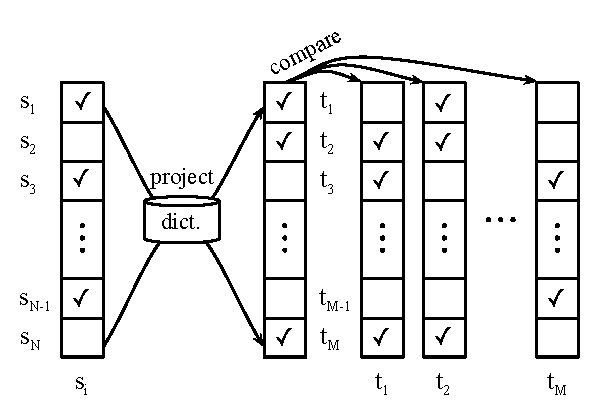
\includegraphics[width=2.8in]{figures/contextual}}}
\caption{Lexicon induction using contextual information. First, contextual vectors are projected using small seed dictionaries and then they are compared with the target language candidates.}
\label{fig:contextual}
\end{figure}

\noindent\emph{Temporal cue} \\

Online content is often published along with temporal information: news feeds, for example, are comprised of news stories annotated with date and time of publication.  The feeds are specialized for the target geographical locations and vary in content across languages.  Still, many events are deemed relevant to multiple audiences and the news stories related to them appear in several languages, although rarely as direct translations of one another.  Words associated with these events will appear with increased frequency in multiple languages around the dates when these events are reported.  \figref{fig:temporal} illustrates this idea with temporal histograms of three English words and their Spanish translations. Such weak synchronicity provides a cue about the relatedness of words across the two languages, and can be exploited to associate them.  In order to score a pair of entities across languages, we can compute the similarity of their temporal signatures.\\

\begin{figure}[h]
\centerline{\mbox{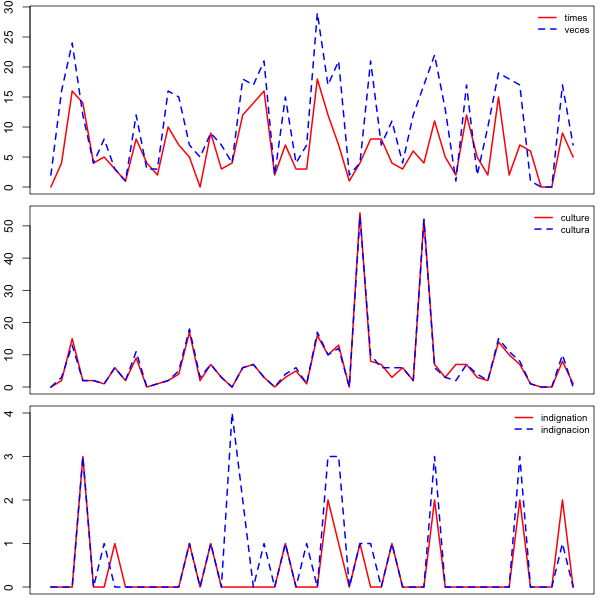
\includegraphics[width=2.8in]{figures/temporal}}}
\caption{Temporal histograms of three English words and their Spanish translations.\todo{From EurPoarl, change fig?}}
\label{fig:temporal}
\end{figure}

\noindent\emph{Orthographic cue} \\

\todo{Edit distance}\\

\noindent\emph{Phonetic cue} \\

\todo{Named entities and cognates.}\\

\noindent\emph{Topic cue} \\

\todo{Wiki categories.}\\

\subsection{Combination Strategies}

These cues provide informative and independent means to score a source word and a target candidate, and combining them is likely to produce better lexicons.  One idea is to directly combine the ranked lists of induced candidates using the mean reciprocal rank (MRR) heuristic frequently used in Information Retrieval literature.  The idea is to score each of the translation candidates with an average reciprocal rank across all rankings, and then sort the candidates in descending order.\\

The relative informativeness of the cues will depend on the data: e.g. the temporal cue depends on the temporal alignment of of both sides of the bilingual corpus, the orthographic cue is uninformative when the two languages use different scripts, etc.  However, the MRR heuristic assigns equal weights to each ranking and investigating more suitable combination strategies remains the subject of ongoing work.\\ 

Some of the metrics we have introduced (e.g. edit distance) are likely to assign same scores to multiple candidates.  We use the following strategy for resolving ties: (1) a set of candidates assigned the same score shares the same rank, (2) a rank assigned to a candidate (a real value) takes into account the number of other candidates with the same or better scores (\figref{fig:rankties}).\\

\begin{figure}
\centerline{\mbox{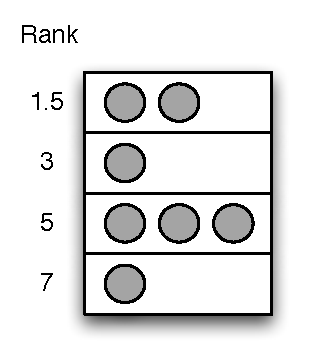
\includegraphics[width=1.3in]{figures/rankties}}}
\caption{Resolving ties.}
\label{fig:rankties}
\end{figure}

\subsection{Handling Morphology} \label{sect:morph}

Many of the languages in our list such as Russian and, Korean are characterized by morphological rules generating a large 
number of word forms for the same lexeme.  Thus, we need to be able to group morphological variants of the same word into an equivalence class and collect their aggregate statistics.  For instance, we would like to count the total number of occurrences of \emph{\{Herzegovina, Hercegovina\}} on the English side in order to map it accurately to the corresponding equivalence class we may see on the Russian side of our corpus (e.g. \cyri{\{Gercegovina, Gercegovinu, Gercegoviny, Gercegovino\U{i}\}}).  In order to keep to our objective of requiring as little language knowledge as possible, we take a rather simplistic approach for grouping equivalence classes.  For morphologically rich languages, a set of words are in the same equivalence class if they share a prefix of size five or longer.  For the other languages, each unique word is assigned its own class.  More sophisticated unsupervised approaches (i.e. \cite{Goldwater:2006}) could be incorporated instead and are a subject of ongoing work.

%-----------------------------------------------------
\section{Resources} \label{sect:resources}

\noindent{\em News wire}\\ 

\todo{Markup removed language identified, and temporal information extracted. Up to 10 years of temporal data for 23 languages. A substantial portion of the collected data still needs to be processed for language and time.}\\

\noindent{\em Wikipedia}\\

\todo{Markup removed, interlingual links used to pair up pages between English and another language.  Done for 43 languages.  Have topic information for the topic similarity cue. To keep them comparable, we extracted pages with interlanguage links - stats.  Table \ref{lang-table} shows our 42 languages of interest and the number of Wikipedia articles with interlingual links to their English counterparts.} \\ 
 
\begin{table}[h]
\small
\begin{center}
\begin{tabular}{cc|cc}
Tigrinya	&	36	&	Punjabi 	&	401	\\ 	
Kyrgyz	&	492	&	Somali 	&	585	\\ 	
Nepali 	&	1293	&	Tibetan	&	1358\\
Uighur	&	1814	&	Maltese 	&	1896\\
Turkmen	&	3137	&	Kazakh 	&	3470\\
Mongolian 	&	4009	&	Tatar	&	4180\\
Kurdish	&	5059	&	Uzbek 	&	5875\\
Kapampangan	&	6827	&	Urdu 	&	7674\\
Irish 	&	9859	&	Azeri	&	12568\\
Tamil	&	13470	&	Albanian 	&	13714\\
Afrikaans	&	14315	&	Hindi 	&	14824\\
Bangla 	&	16026	&	Tagalog	&	17757\\
Latvian	&	22737	&	Bosnian 	&	23144\\
Welsh	&	25292	&	Latin 	&	31195\\
Basque 	&	38594	&	Thai	&	40182\\
Farsi	&	58651	&	Bulgarian 	&	68446\\
Serbian	&	71018	&	Indonesian 	&	73962\\
Slovak 	&	76421	&	Korean	&	84385\\
Turkish 	&	86277	&	Ukrainan	&	91022\\
Romanian 	&	97351	&	Russian	&	295944\\
Spanish 	&	371130	&	Polish	&	438053\\

\end{tabular}
\end{center}
\normalsize
\caption{Our 42 languages of interest and the number of Wikipedia pages for each that have interlanguage links with English.\todo{add dictionary info and coverage}}
\label{lang-table}
\end{table}
 
\noindent{\em Dictionaries and stopword lists}\\ 

\todo{Talk about the fact that they are noisy, romanized.  Evaluation results are conservative.  \todo{Include wiki src/trg dictionary coverage, and whether or not useful directly (e.g. romanized)}}\\

\noindent{\em Parallel texts}\\

\todo{MT Workshop data, some are time stamped.  We use one language pair to figure an upper bound. How many days and tokens.}\\

%\begin{table}[h]
%\begin{center}
%%\small
%%\vspace{-.75cm}
%\begin{tabular}{lrrr | lrrr}
%Language	&	Dictionary	&	Wikipedia 	&Newswire&	Language	&	Dictionary	&	Wikipedia & Newswire	\\
%&	entries	&	words (est.)	&words&&		entries &words		&	words\\
%\hline
%Polish	&	261,463	&	249,000,000	&&	Uzbek	&	190,688	&	3,100,000	 &\\
%Russian	&	423,009	&	149,000,000	&&	Maori	&	27,967	&	2,900,000	 &\\
%Ukrainian	&	14,056	&	59,000,000	&&	Kapampangan	&	1,000	&	2,800,000	 &\\
%Turkish	&	1,272,881	&	54,000,000	&&	Tatar	&	8,557	&	1,700,000	\\
%Romanian	&	249,479	&	53,000,000	&&	Kazakh	&	145,750	&	1,300,000	&\\
%Slovak	&	233,093	&	46,000,000	&&	Nepali	&	6,812	&	1,200,000		&\\
%Indonesian	&	67,633	&	42,000,000	&&	Maltese	&	7,574	&	1,000,000	&\\
%Korean	&	229,742	&	36,000,000	&&	Mongolian	&	948	&	800,000	&\\
%Serbian	&	168,140	&	31,000,000	&&	Turkmen	&	91,928	&	500,000	&\\
%Bulgarian	&	316,631	&	29,000,000	&&	Kirghiz	&	74,890	&	300,000	&\\
%Farsi/Persian	&	198,605	&	23,000,000	&&	Somali	&	230	&	200,000	&\\
%Thai	&	14,925	&	18,000,000	&&	Punjabi	&	76,311	&	180,000	&\\
%Basque	&	880	&	14,000,000	&&	Tibetan	&	59,083	&	110,000	&\\
%Malaysian	&	9,438	&	14,000,000	&&	Tigrinya	&	56	&	80,000	&\\
%Bosnian	&	18,283	&	11,000,000	&&	Uighur	&	16,285	&	80,000	&\\
%Latin	&	18,884	&	11,000,000	&&		&		&		&\\
%Hindi	&	58,179	&	10,000,000	&&	German	&	272,230	&	372,000,000	&\\
%Albanian	&	188,563	&	9,800,000	&&	French	&	195,627	&	327,000,000	&\\
%Azeri	&	231,891	&	9,200,000	&&	Italian	&	166,966	&	232,000,000	&\\
%Tagalog	&	247,662	&	9,100,000	&&	Dutch	&	233,805	&	224,000,000	&\\
%Welsh	&	25,832	&	9,000,000	&&	Portuguese	&	840	&	198,000,000	&\\
%Bangla	&	1,606	&	8,400,000	&&	Spanish	&	347,441	&	188,000,000	&\\
%Latvian	&	148,363	&	8,200,000	&&	Swedish	&	227,849	&	134,000,000	&\\
%Tamil	&	165,004	&	7,200,000	&&	Chinese	&	82,080	&	95,000,000	&\\
%Kurdish	&	9,870	&	5,400,000	&&	Czech	&	262,690	&	50,000,000	&\\
%Afrikaans	&	11,389	&	5,000,000	&&	Hungarian	&	289,225	&	50,000,000	&\\
%Urdu	&	36,428	&	4,100,000	&&	Arabic	&	167,189	&	37,000,000	&\\
%Irish	&	887	&	3,400,000	&&	Greek	&	160,126	&	17,000,000	&\\
%\end{tabular}
%%\normalsize
%\end{center}
%\caption{The number of entries in the bilingual dictionaries assembled at JHU, estimated number of words contained in each of the language-specific versions of Wikipedia, and the number of words contained in each of the collected newswire datrasets.  The languages which have been extensively studied in statistical machine translation literature are given in the lower right corner. }\label{fig:datastats}
%\end{table}

%-----------------------------------------------------
\section{Experimental Evaluation}

We evaluate performance of the lexicon induction framework on the monolingual resources we have collected and described in \secref{sect:resources}.  In the first set of experiments, we consider a high resource language pair to establish relative efficacy of the cues and to get a sense of an upper bound on the overall performance. We then induce translations between English and each of the low resource languages of interest.  Since many of the seed and test dictionaries are sparse and noisy, we investigate the feasibility of crowd-sourcing annotations and their use in an iterative induction procedure.  Finally, we investigate heuristics we discussed in \label{sect:morph} for handling morphology.\\

In each experiment, we use $10\%$ of the dictionary to test the induced candidate lists for 1000 source words.  Unless mentioned otherwise, we use the simple equivalence class heuristic (i.e. each unique token is assigned its own equivalence class) when constructing both contextual vectors and candidates.  The performance is measured by top-$k$ accuracy, i.e. the proportion of source equivalence classes which have at least one test dictionary translation among top $k$ of its induced candidates.  Note that the reported performance is conservative since the test dictionaries are both noisy and sparse.\\

As we have pointed out, one of the objectives of this work is to induce lexicons with wide coverage.  Thus, unlike most of the previous work, we are particularly interested in inducing translations for source equivalence classes \emph{randomly} selected from the test dictionary. 

\subsection{Lexicon induction for a high-resource language pair}

We begin by evaluating the relative performance of lexicons induced from contextual, temporal, and orthographic cues as well as the MRR rank aggregation scheme on the English-Spanish EuroParl parallel data  for inducing translations for a \emph{random} 1000 words in our test dictionary (\figref{fig:exp1}, top).  The corpus is time stamped (spanning 656 days) and perfectly \emph{temporally} aligned, so it is not surprising that the temporal cue provides a strong signal for inducing translations.  All of these cues are informative and orthogonal, so combining them substantially improves results with $70\%$ and  $79\%$ accuracy at top 100 and 500, respectively.  \\

\begin{figure}[h!]
\centerline{\mbox{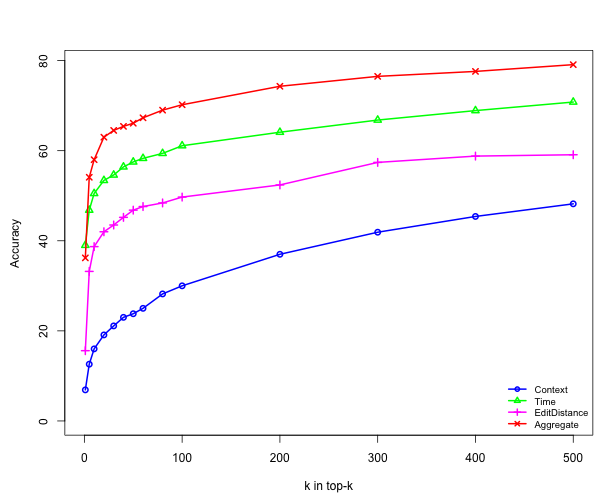
\includegraphics[width=3in]{figures/exp1/parallel.rand/parallel}}}
\centerline{\mbox{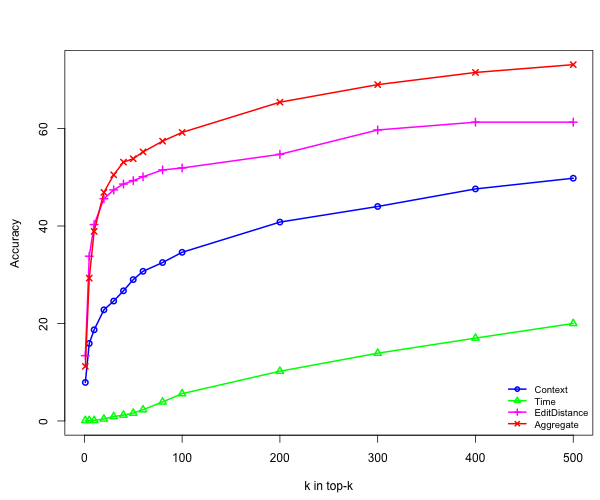
\includegraphics[width=3in]{figures/exp1/wikinews.rand/wikinews}}}
\caption{Relative accuracy on parallel en-es data (top), and wikipedia / newswire (bottom) $\leftarrow$ \todo{replace with random} for 1000 random source words.}
\label{fig:exp1}
\end{figure}

We repeat the same experiment using wikipedia and newswire data to derive dictionaries from contextual and temporal cues, respectively (\figref{fig:exp1}, bottom).  Since the newswire corpora is only weakly temporally aligned, the performance of the temporal cue drops substantially.  Still, the cues provide informative and non-redundant signals, which can be combined to obtain better quality lexicons.

\subsection{Context vs.\ alignments} 

Word alignments can be induced directly from sentence aligned corpora.  In this set of experiments, we compare bilingual lexicons derived from word alignments (produced by GIZA++) to those generated from the contextual cue alone on the English-Spanish section of the EuroParl corpus (see \figref{fig:exp2}).  Unsurprisingly, word alignments induce a much more informative signal than context alone, but sufficient sentence aligned bilingual data is not available for most of the low resource languages we consider in this work.\\

\begin{figure}[h!]
\centerline{\mbox{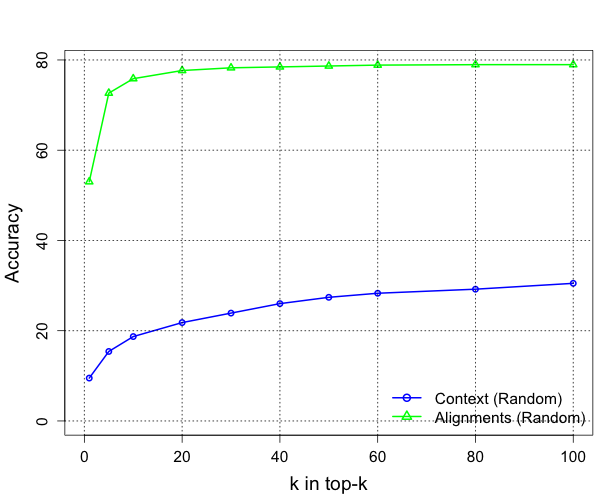
\includegraphics[width=3in]{figures/exp2/alignvscontext}}}
\caption{Relative accuracy of lexicons induced from alignments and context on parallel en-es data for random and most frequent 1000 source words.}
\label{fig:exp2}
\end{figure}

We also compare the induced lexicon accuracy for random and most frequent 1000 source words.  The substantial gap in performance highlights that evaluating on most frequent source words alone can be misleading if the objective is to induce wide coverage dictionaries.

\subsection{Lexicon induction for a low-resource languages}

\todo{Candidates and context from wiki, and time from newswire for (18?) languages and English.}

\subsection{Crowd-sourcing annotation}

We use our existing bilingual dictionaries to induce large bilingual lexicons via the contextual cue and to evaluate their accuracy.  However, these dictionaries vary substantially in quality and coverage across languages and corpora (see \secref{sect:resources}).  In this set of experiments we study \cite{Irvine:2010} the viability of crown-sourcing translations for a low-resource languages specifically for use in our induction framework.  First, we use the contextual cue to induce lexical translation pairs from the Wikipedia monolingual data. Then, we pay Amazon Mechanical Turk (MTurk) workers a small amount to check and correct our system output. We can then use the updated lexicons to inform another iteration of lexicon induction, gather a second set of MTurk annotations, and so on. \\

For 32 of the 42 languages in \tabref{lang-table}, we were able to induce lexical translation candidates and post them on MTurk for annotation. For these languages we presented annotators with top ten scored candidates for a set of 100 English words and asked them to mark correct translations. If our seed dictionary included an entry for a source word, we included the translation in the candidate list as a positive control. Additionally, we included a random word in the foreign language as a negative control.  We do not have dictionaries for the remaining 10 languages, so we asked workers to type translations for 100 English words. We had three distinct workers provide such annotations for each source word. \\ 

\begin{figure}[h!]
\centerline{\mbox{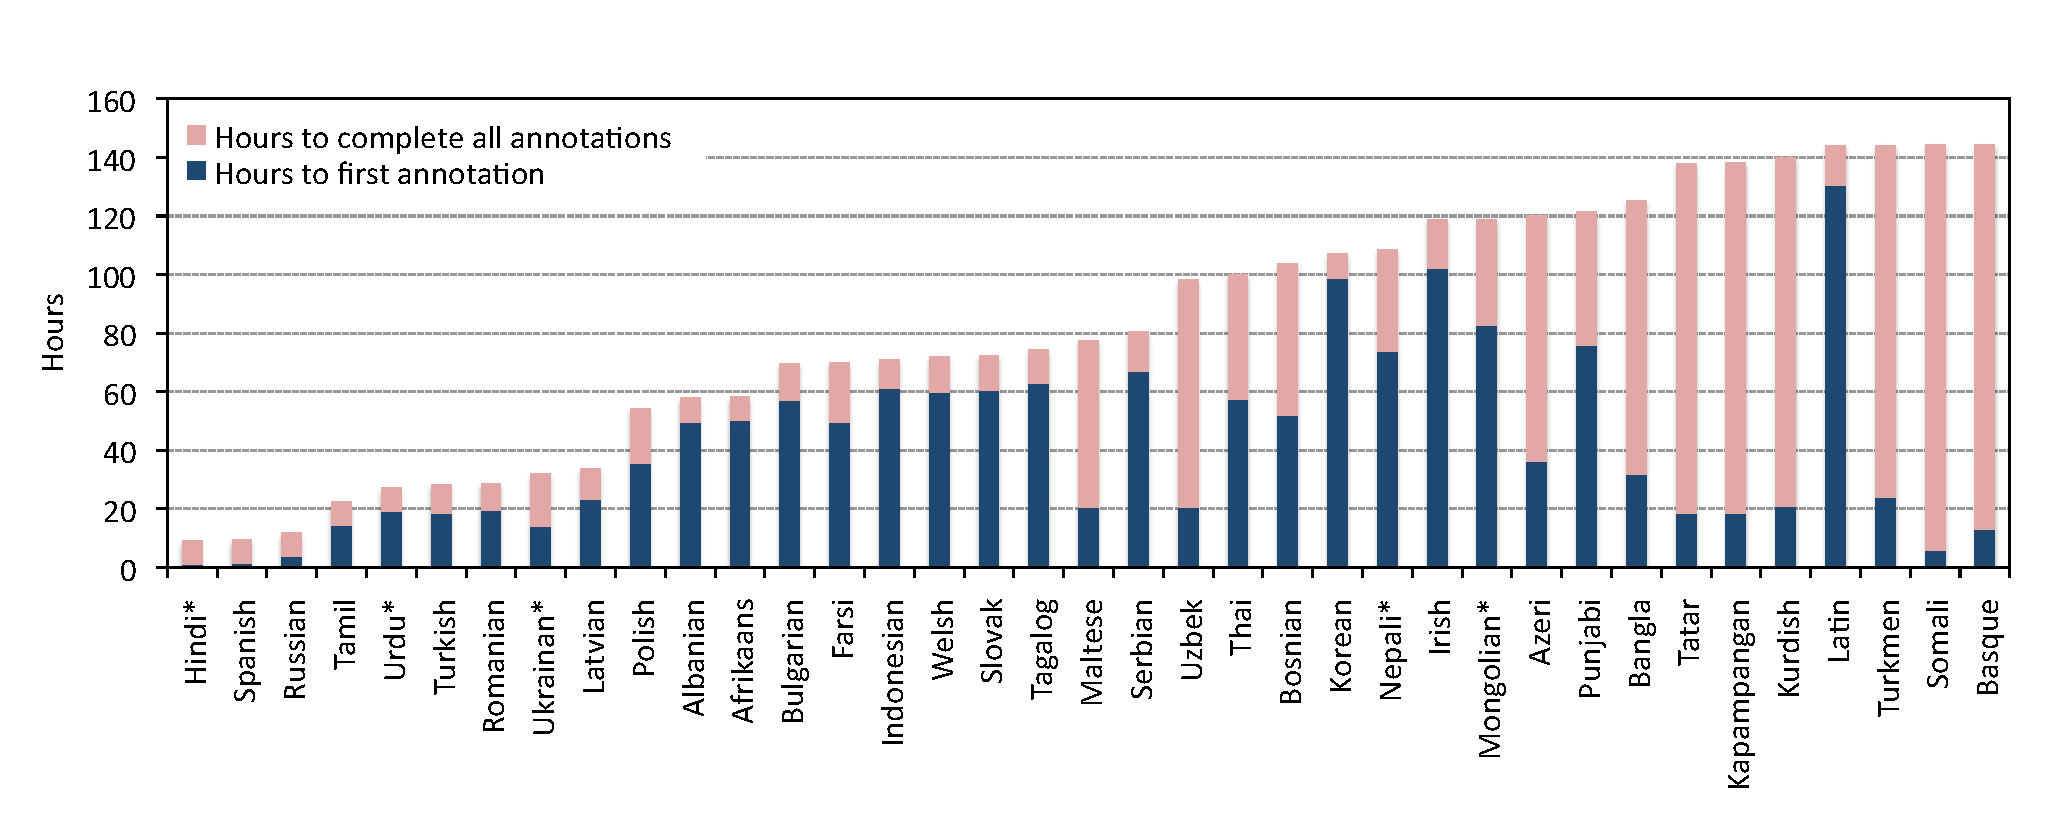
\includegraphics[width=5in]{figures/exp4/time}}}
\centerline{\mbox{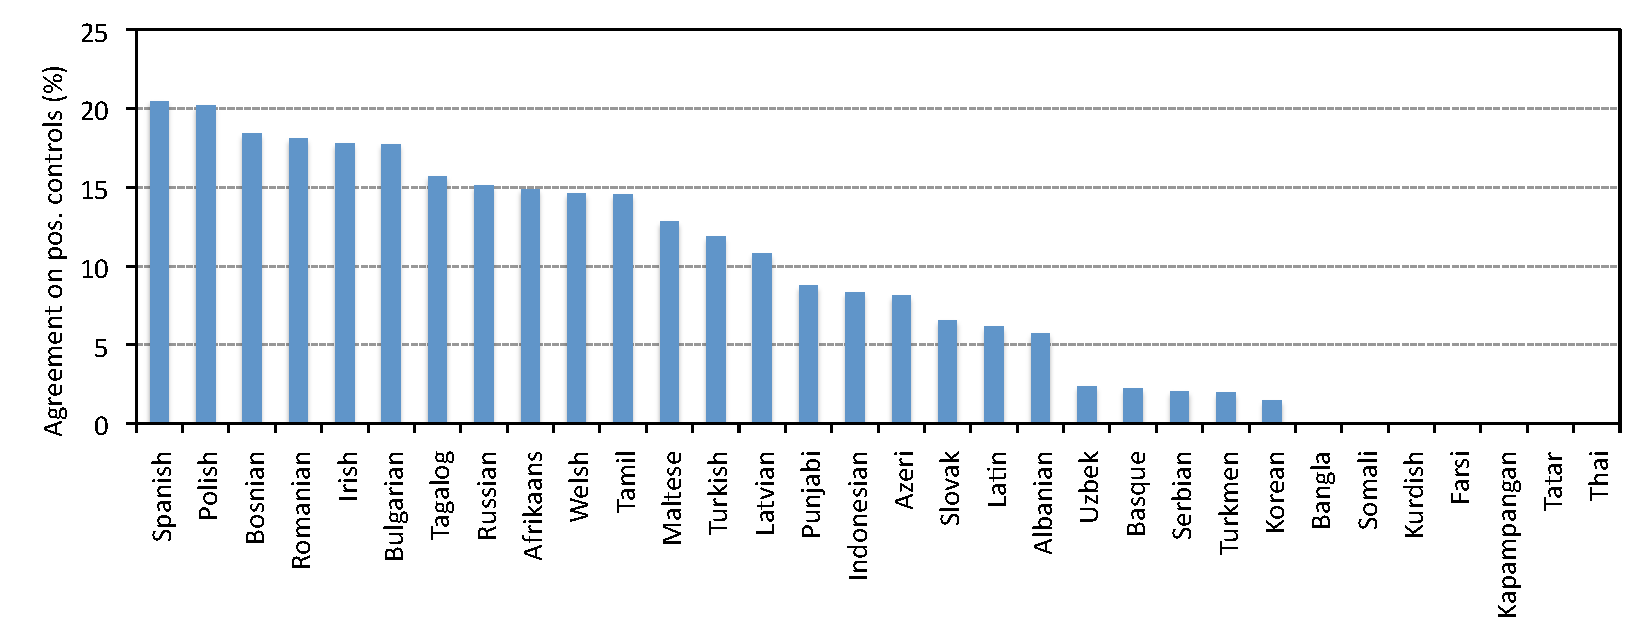
\includegraphics[width=5in]{figures/exp4/controls}}}
\caption{Top: time to complete annotation of 100 English words.  Division of the time between posting and the completion of the first annotation unit (HIT) and the time between the completion of the first and last HIT shown. HITs that required lexical translation only are marked with an $*$. Bottom: percent of positive control candidate translations for which two or three workers checked as accurate.}
\label{fig:exp4}
\end{figure}

\figref{fig:exp4} (top) shows the time it took to complete annotation of for 37 languages on MTurk. Annotations the following languages were posted for a week and were never completed: Tigrinya, Uighur, Tibetan, Kyrgyz, and Kazakh. All five of the uncompleted required typing annotations, a more time consuming task than checking translation candidates. Not surprisingly, languages with many speakers (Hindi, Spanish, and Russian) and languages spoken in and near India (Hindi, Tamil, Urdu) were completed very quickly. \figref{fig:exp4} (bottom) shows the percent of positive control candidate translations that were checked by the majority of workers (at least two of three). The highest amounts of agreement with the controls were for Spanish and Polish, which indicates that those workers completed the annotations more accurately than the workers who completed, for example, the Tatar and Thai annotations. However, the seed dictionaries are very noisy, so this finding may be confounded by discrepancies in the quality of our dictionaries. The noisy dictionaries also explain why agreement with the positive controls is, in general, relatively low.\\

To understand the utility of MTurk generated translation for inducing lexicons, we supplemented our dictionaries for each of the 37 languages for which we gathered MTurk annotations with translation pairs that workers agreed were good (both chosen from the candidate set and manually translated). We compared seed dictionaries of size 200 with those supplemented with, on average, 69 translation pairs. We found an average relative increase in accuracy of our output candidate set (evaluated against complete available dictionaries) of {\bf 53\%}.\\

In sum, we found that the iterative approach of automatically generating noisy annotation and asking MTurk users to correct it to be an effective means of obtaining supervision.  These correction tasks are simple, can be completed quickly for a large number of low resource languages, and produce high quality annotation.

\subsection{Dealing with morphology}

\todo{Morphological equivalence classes for context and source/target candidates.}

%-----------------------------------------------------
\section{System Overview}

In this section we touch on some of the implementation details of the lexicon induction framework: we overview the data collection and lexicon induction procedures and explain how the framework can be extended to include new monolingual resources and cues derived from them.  

\subsection{Data Collection}

While some monolingual resources (see \secref{sect:resources}) are static, others require ongoing collection.  We have set up the nutch crawler\footnote{http://nutch.apache.org/} to continuously crawl a number of web sites generating news content in the languages of interest.  The crawl results are periodically processed (see \figref{fig:data}) to (1) parse page content and extract metadata associated with the page, (2) merge with previously extracted pages, (3) identify language of the page content, and (4) generate time annotated corpora for each of the languages.  See \tabref{fig:datastats} for a current summary of the collected data.

\begin{figure}[h]
\centerline{\mbox{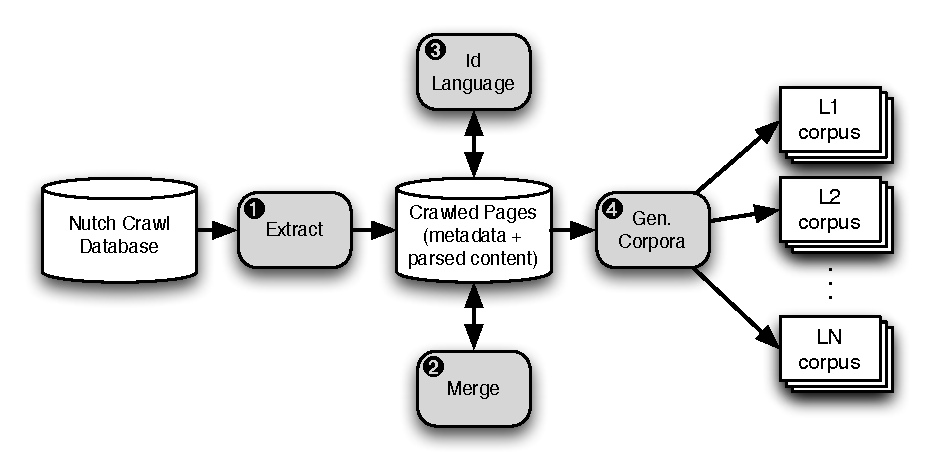
\includegraphics[width=3in]{figures/datacollect}}}
\caption{Ongoing data collection.}
\label{fig:data}
\end{figure}

\subsection{Lexicon Induction Procedure}

Let us turn to the induction procedure, highlight some of the most relevant code, and show how the framework can be extended to include new monolingual resources and cues.  \figref{fig:packages} shows the implementation layout and \figref{fig:system} gives a high level view of the lexicon induction procedure.\\

\begin{figure}[h]
\centerline{\mbox{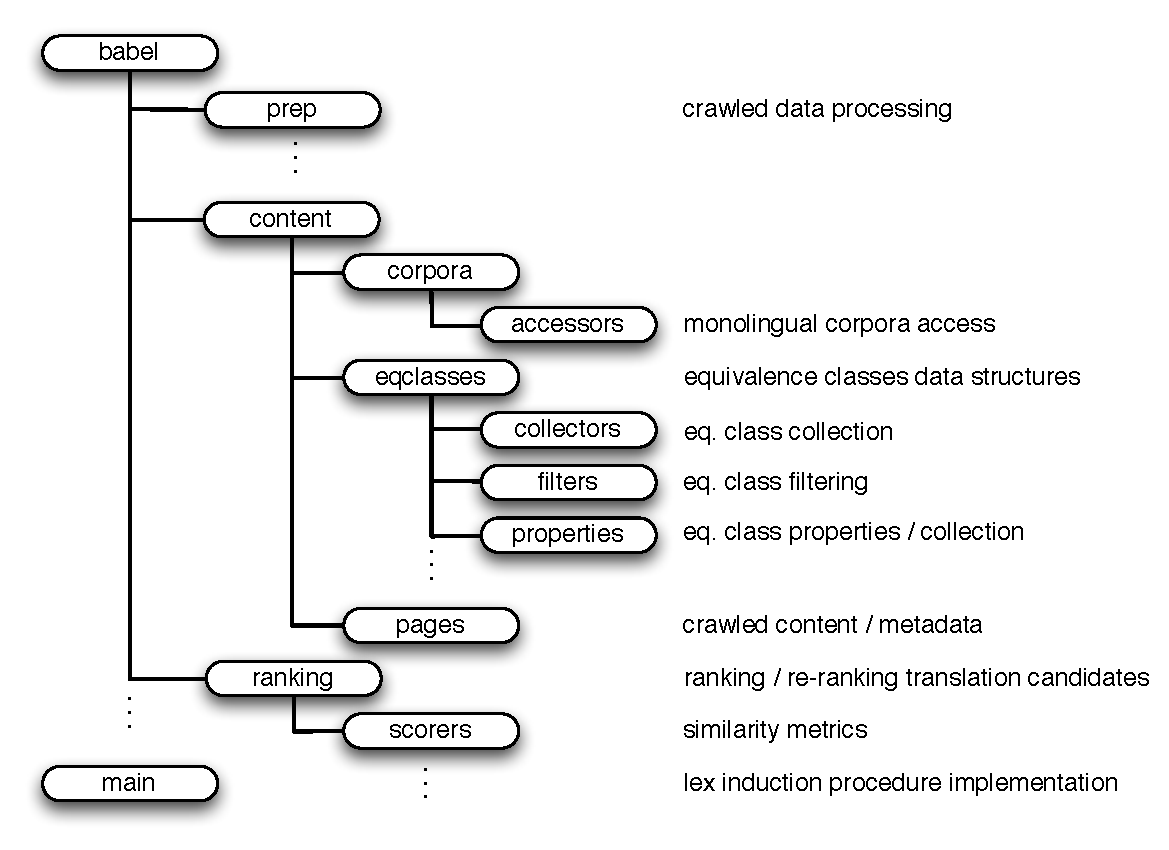
\includegraphics[width=3in]{figures/packages}}}
\caption{Implementation layout of the lexicon induction framework.}
\label{fig:packages}
\end{figure}

We argued in \secref{sect:morph} that collecting aggregate statistics for morphological variants of a single lexeme is important when dealing with morphologically rich languages.   Base class \small{\tt EquivalenceClass} groups morphological variants present in the data into equivalence classes and maintains a set of aggregate statistics derived from monolingual cues.  In turn, each of the statistics, or properties, is implemented by a subclass of \small{\tt Property}. \\

\begin{figure}[h!]
\centerline{\mbox{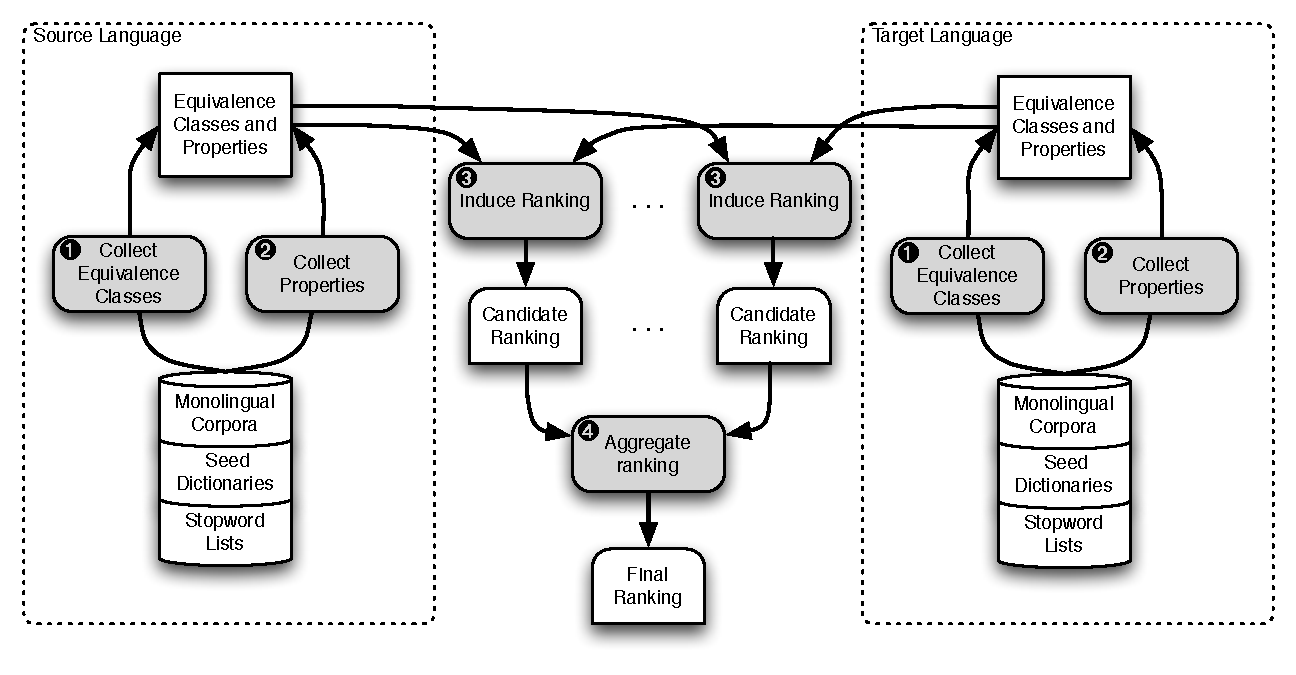
\includegraphics[width=4in]{figures/lexinduct}}}
\caption{A high level overview of the lexicon induction framework.  Equivalence classes and corresponding properties are first extracted from monolingual data (steps 1 and 2).  Similarity metrics defined over the properties are then used top produce rankings over target candidates in step 3.  Finally, ranked lists are aggregated to produce the final rankings in step 4.}
\label{fig:system}
\end{figure}

The induction procedure begins with two passes through both source and target language monolingual corpora (step 1 and 2 on \figref{fig:system}, respectively) implemented in \small{\tt DataPreparer}.  Each of the available corpora (e.g. see \secref{sect:resources}) is accessed through a corresponding subclass of \small{\tt CorpusAccessor}.  In the first pass, morphological variants are collected (see \small{\tt EquivalenceClassCollector}) to generate the corresponding equivalence classes and, in the second pass, a set of properties such as contextual vectors, temporal distributions, topic information, etc.\ is collected for each of the equivalence classes. The initial set of equivalence classes is pruned by a series of filters extending \small{\tt EquivalenceClassFilter} in order to throw out patently incorrect or undesirable candidates, e.g. stop words, least or most frequent classes, strings containing numbers or letters of a wrong script, etc. Both source and target equivalence classes along with the collected statistics are persisted on disk.\\

Next, collected properties along with the corresponding similarity metrics extending \small{\tt Scorer} are used to produce a ranked list of candidates for each of the source equivalence classes.  This step involves a substantial amount of computation since each of the source equivalence classes is compared with all of the target candidates. Its implementation in \small{\tt Ranker} is parallelized, which substantially speeds up this step.  Ranked candidate lists induced for each source equivalence class from multiple cues are aggregated (see \small{\tt Reranker}) into a joint ranking in step 4 on \figref{fig:system}  Finally, the induced ranked candidate lists are evaluated in \small{\tt NBestCollector}.\\

\lstref{fig:cfg} shows an example configuration file for setting up the induction process.  It is split into 5 sections, one would:

\begin{itemize}
  \item The \small{\tt  corpora} section lists both source and target monolingual corpora with additional configuration parameters specific to the corresponding subclass of \small{\tt CorpusAccessor}.
  \item The \small{\tt  resources} section specifies additional resources, such as stop word lists and bilingual dictionaries.
  \item The \small{\tt  preprocessing} section configures the two stage preprocessing stage, i.e. which resources to use to generate equivalence classes and how to collect their properties.  For example, the \small{\tt  candidates} section on \lstref{fig:cfg} specifies that the simple and prefix heuristics (see \secref{sect:morph}) should be used for generating source and target equivalence classes, respectively, and that the classes should be pruned if they occur fewer than 10 times in the data.
  \item Finally, the \small{\tt experiments} section configures the induction process.  The configuration parameters can be used to choose most frequent or random source equivalence classes for induction (\small{\tt RandomSource}), the portion of the dictionary to use for projecting contextual vectors (\small{\tt DictionaryPercentToUse}), the target candidate ranked lists size to induce  (\small{\tt NumTranslationsToAddPerSource}), the number of threads to use when generating rankings (\small{\tt NumRankingThreads}), and to specify which properties are to be used to induce those rankings and whether or not to aggregate them (\small{\tt DoAggregate}).\\
\end{itemize}

In order to extend the framework to add a new monolingual resource and/or include additional cues:

\begin{itemize}
  \item Extend \small{\tt CorpusAccessor} to enable access to a new resource.
  \item Extend \small{\tt Property} and \small{\tt PropertyCollector} to manage and collect desired statistics from a monolingual resource.
  \item Extend \small{\tt Scorer} to implement a similarity metric for scoring a source and a target candidate equivalence classes.
\end{itemize}

\newpage
\lstinputlisting[caption=Example configuration file.,label=fig:cfg]{figures/babel.xml}
\newpage

%-----------------------------------------------------
\section{Future Work}

\begin{itemize}
  \item MT
  \item Dealing with noisy dictionaries
  \item Better combination strategies
\end{itemize}

%-----------------------------------------------------
\section{Conclusions}

\bibliographystyle{apalike}
\bibliography{references}
 
\end{document}
